\section{Existant Organisationnel}
    \subsection{Structure Organisationnel de GSTP}

		L'entreprise GSTP est centrée autour d'un siège social, il regroupe six directions :
	    \begin{itemize}
            \item Direction générale
            \item Direction générale (DG)
			\item Direction des ressources humaines (DRH)
			\item Direction des finances et comptabilité (DFC)
			\item Direction informatique (DI)
			\item Direction du matériel (DM)
			\item Direction travaux, études et méthodes (DTEM).
        \end{itemize}
        L'entreprise possède environ une quarantaine de chantiers autonomes. Étant donné que le champ d'action se porte sur un rayon d'environ 500 km, il peut entrainer des difficultés logistiques et de transport de matériel.

		% ORGANIGRAMME
		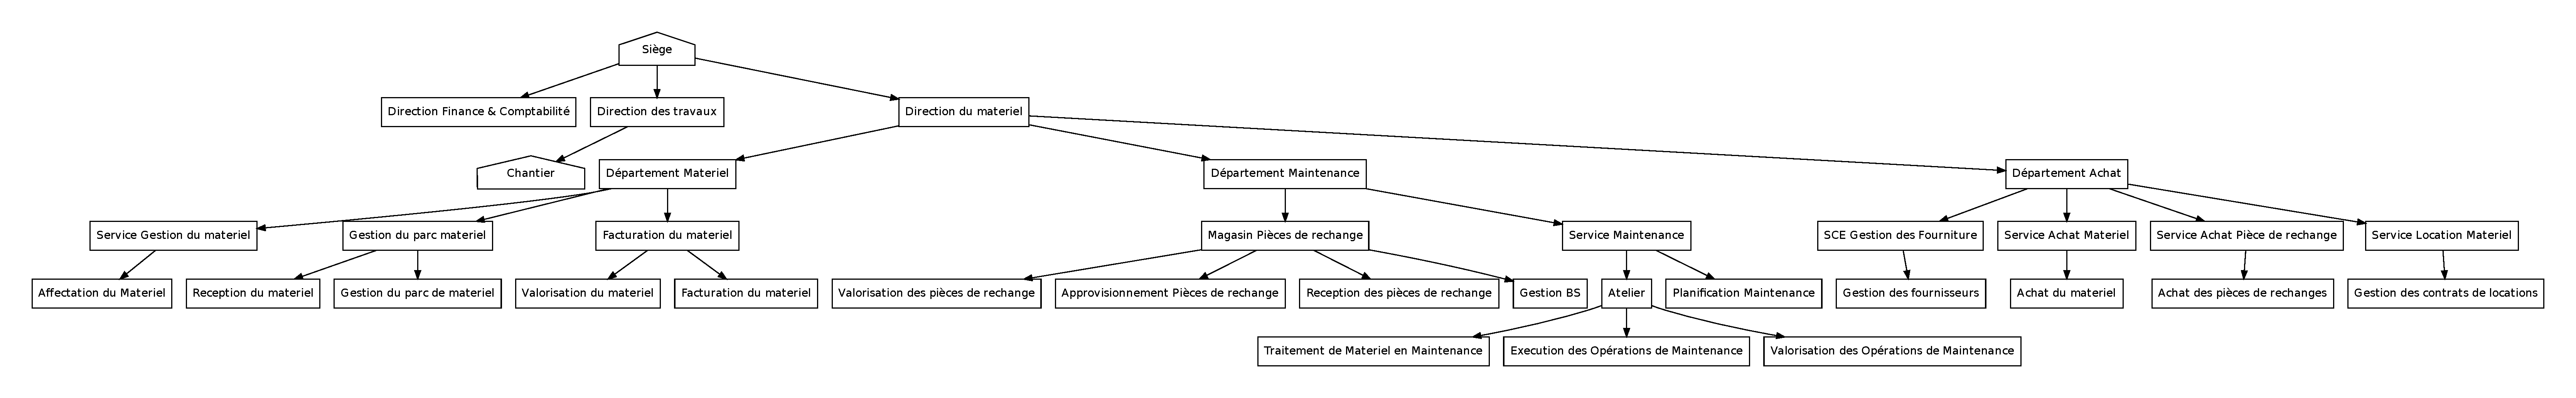
\includegraphics[width=\textwidth]{img/structureOrganisationnel.pdf} 
		
    \subsection{Direction du Matériel (DM)}
            Rattachée à la direction générale, la direction du matériel a pour missions de :
            \begin{itemize}
                \item affecter le matériel aux chantiers.
                \item assurer la maintenance et la rénovation du matériel.
                \item gérer le stock de pièces de rechange.
                \item renouveler le matériel (acquisition), avec l'accord de la DG car il s'agit d'un acte d'investissement.
                \item facturer l'utilisation du matériel aux chantiers. La DM joue un rôle de fournisseur (location du matériel) vis-à-vis des chantiers.
            \end{itemize}
            
        \subsubsection{Les Départements et leur rôles}
            \paragraph{Département Matériel}
                Le département matériel est composé de trois services :
                \subparagraph{Service de Gestion du Matériel}
                    Son rôle est de gérer le planning d'affectation et d'assurer l'affectation du matériel aux différents chantiers. Il est constitué de trois personnes.
                \subparagraph{Service de Gestion du Parc Matériel}
                    Il s'occupe de la réception, envoi du matériel et de la gestion du parc matériel. Il est constitué d'une personne.
                \subparagraph{Service de Facturation du Matériel}
                    Ce service s'occupe de la valorisation et de la facturation du matériel. Il est constitué d'une personne.        
                
            \paragraph{Departement Maintenance}
                Il est composé de deux services :
                \subparagraph{Service de Gestion des Pièces de Rechange}
                    Son rôle est d'assurer l'approvisionnement, la réception, la valorisation et la gestion des pièces   de rechange. Il y a un magasin au siège de l'entreprise et deux autres délocalisés. Ce service est constitué d'une personne par magasin. 
                \subparagraph{Service de Maintenance}
                    Il est composé d'une quarantaine d'ateliers et il s'occupe de la planification, de l'exécution et de la valorisation des opérations de maintenance et des divers traitements. Ce service est constitué de 60 personnes répartis sur 40 ateliers (dont 8 à l'atelier principal, et les autres étant repartis sur les ateliers de chantiers).

            \paragraph{Département Achat}
                Le département achat est constitué de quatre services :

                \subparagraph{Service de Gestion des Fournisseurs}
	                C'est le service qui va être en communication avec les fournisseurs de matériel afin d'avoir les meilleurs matériels sur le marché aux moindres coûts.
                \subparagraph{Service d'Achat du Matériel}
	                Ce service s'occupe des achats de nouveaux matériels.
                \subparagraph{Service d'Achat des pièces de Rechange}
	                Ce service s'occupe de tous les achats de pièces de rechange.
                \subparagraph{Service de Location du Matériel}
	                Ce service s'occupe des locations de matériels lorsque le parc n'offre pas suffisamment de disponibilités pour répondre à un besoin d'un chantier. Il peut également s'occuper de l'achat d'autres prestations (maintenance, etc.)


\section{Processus stratégiques}
		La direction matériel de GSTP repose sur 5 principaux processus :
		\begin{itemize}
				\item Processus d'approvisionnement de pièces de rechange
				\item Processus de facturation du matériel pour un chantier
				\item Processus d'affectation et de restitution du matériel
				\item Processus de maintenance du matériel
				\item Processus de planification de l'affectation du matériel
    \end{itemize}


		\subsection{Processus d'approvisionnement de pièces de rechange}
				\subsubsection{Description}
				
						L'approvisionnement des pièces de rechange se déroule suivant le cycle suivant :
						\begin{itemize}
						    \item D'abord on calcule le stock des pièces de rechange à chaque fois que l'on fait l'inventaire mensuel des pièces de rechange ou lorsque l'on reçoit des pièces de rechange, ou lorsqu'une pièce de rechange sort du stock (magasin).
						    \item On produit ainsi la variation de stock qui, associée aux prévisions de consommation nous conduit à calculer les besoins en piéces de rechange. Un calcul des besoins est également fait mensuellement. Le calcul des nouveaux besoins donne suite à l'édition d'une demande de réapprovisionnement en pièces de rechange.
						    \item Enfin on transmet cette demande de réapprovisionnement (ou une demande urgente d'approvisionnement
établie par un des chantiers), cela aura pour effet de produire une commande de pièces de rechange par le département Achat.
						\end{itemize}
						
				%\subsubsection{MCD}
				
				%\subsubsection{MCT}
				
				%\subsubsection{MOT}
				
		\subsection{Processus de facturation du matériel pour un chantier}
				\subsubsection{Description}
				
				Cette procédure permet de facturer en interne le matériel sur les différents chantiers. Cette tâche n'est pas assurée par le service Achat car celui-ci ne s'occupe que des factures extérieures.
				\newline
				L'edition de la facturation d'utilisation du matériel par les chantiers est calculée par le service
Facturation Matériel du département Matériel en fonction du :
				\begin{itemize}
						    \item Relevé mensuel du fonctionnement du matériel (RMFM) établi par les chantiers,
						    \item Relevé mensuel des heures de main d'œuvre (RMHMO) établi par le service Maintenance
du département Maintenance,
						    \item Relevé mensuel de consommation de pièces de rechange et pneus (RMCPR) établi par le Service de Gestion de Pièces de Rechange du département Maintenance,
						    \item des frais de gestion, de la masse salariale et du cout de l'heure de main d'œuvre de la
direction de Matériel (DM), renseignements fournis par la direction des Finances et Comptabilité (DFC).
				\end{itemize}
				
				%\subsubsection{MCD}
				
				%\subsubsection{MCT}
				
				%\subsubsection{MOT}

		\subsection{Processus d'affectation et de restitution du matériel}
				\subsubsection{Description}
				
				Cette procédure gère la présence de matériel sur site depuis sa réception auprès du fournisseur jusqu'à son retour du chantier.
				\newline
				La procédure d'affectation s'effectue généralement sur la base du planning d'affectation qui correspond aux prévisions d'utilisation du matériel établi par le DTEM. D'autres demandes, non prévues au planning, sont émises par les chantiers. Ces demandes sont satisfaites, notamment par la sous-traitance. 
				\newline
				En effet, si un matériel venait à manquer, l'entreprise effectue des locations auprès d'entreprises spécialisées dans la location de matériel BTP. Lorsque le matériel n'est plus nécessaire sur le chantier, un avis de restitution de matériel est envoyé, on contrôle l'état du matériel; s'il est en bon état, une demande d'entrée est demandée au service de Gestion du parc matériel; s'il était en location, il est dirigé vers le service location du matériel; et s'il est en panne, une demande de maintenance est faite au service Maintenance.


				%\subsubsection{MCD}
				
				%\subsubsection{MCT}
				
				%\subsubsection{MOT}
				
		\subsection{Processus de maintenance du matériel}
				\subsubsection{Description}
				
				Le département de gestion de la maintenance se charge de la maintenance préventive du matériel (révisions é la restitution par un chantier ou selon le planning de maintenance), et de sa rénovation. Lorsqu'il y a une panne, elle peut être diagnostiquée sur place pour savoir s'il faut réparer sur le chantier ou rapatrier le matériel au siège.
				\newline
				Le service de gestion de la maintenance s'occupe de planifier les opérations de maintenance, les exécuter. Elle est composée de soixante personnes réparties sur quarante ateliers. Huit d'entre elles sont sur l'atelier principal, et le reste sur les ateliers de chantier. Lorsqu'une opération de maintenance est lancée, des personnes sont affectées et des pièces de rechange sont commandés, puis la réparation est effectuée. A la fin de chaque opération de maintenance un avis de maintenance est émis au département maintenance ou au chantier concerné.
				
				%\subsubsection{MCD}
				
				%\subsubsection{MCT}
				
				%\subsubsection{MOT}
				
		\subsection{Processus de planification des affectation du matériel}
				\subsubsection{Description}
				
				Ce processus est très transverse aux départements et services de la direction matériel.
				Parmi les services qui réalisent la planification, il y a : ceux du département achats (les services d'achat du matériel, d'achat de pièces de rechanges et location du matériel), ceux également des départements matériel et maintenance.
				\newline
				Le département du matériel planifie l'utilisation de matériels par les chantiers et leurs affectations aux chantiers. Elle s'occupe d'envoyer aux départements achat et maintenance les demandes de matériel par chantier : demande de location ou d'achat de nouveau matériel et planification des opérations de maintenance du matériel sur site.
				\newline
				Le département d'achat du matériel prévoit un planning de commande de matériel et la location de celui-ci. 
				\newline
				Le département de maintenance planifie la maintenance, la disponibilité du personnel et la consommation de pièces de rechange.
				
				%\subsubsection{MCD}
				
				%\subsubsection{MCT}
				
				%\subsubsection{MOT}

\section{Existant informatique}

		Actuellement, 30 chantiers effectuent leur pointage manuel et ensuite les transmettent au siège. Seuls 10
chantiers sont équipés d'ordinateurs. L'entreprise prévoit d'équiper l'ensemble des chantiers sur un horizon de 10 mois. 
Ces outils informatiques permettent la saisie et la transmission des données de gestion vers le siège.
		Au siège, il y a 60 postes et une imprimante principale.
		
		\subsection{Niveau logiciel}
		
		Au niveau de la direction du matériel, l'architecture logicielle regroupe plusieurs applications.
Chaque département de la DM possède des applications en interne et indépendantes qui reposent sur des fichiers. Aucun système informatique
ne permet la centralisation de ces informations.

		\begin{description}
			\item[Département Matériel :] possède une application de gestion du planning ainsi qu'une application de facturation.
			\item[Département Maintenance :] dispose d'un logiciel de gestion de stocks et pièces de rechange, et d'un autre de planification de maintenance
			\item[Département Achat :] possède une applications de gestion des fournisseurs (300 environ), d'une autre de gestion de bons de commande.
		\end{description}


		\subsection{Niveau matériel}

		 L'architecture matérielle de la DM n'est pas très développée.

		\begin{description}
			\item[Département Matériel :] est doté de 3 postes et 2 imprimantes.
			\item[Département Maintenance :] est doté de 2 postes et 2 imprimantes
			\item[Département Achat :] est doté de 2 postes et 2 imprimantes
		\end{description}
		
		
		
\section{Dysfonctionnements}	
		
		Au niveau de l'existant organisationnel, les dysfonctionnements détectés sont :
		
		\subsection{Département Matériel}
				\begin{itemize}
						\item Mauvaise planification des affectations du matériel car le dispositif de pointage ne permet pas d'avoir une vision globale du planning.
						\item Immobilisation du matériel car le système actuel ne permet pas de repérer en temps réel la sous-exploitation d'un matériel.
						\item L'utilisation du papier, en plus d'être un moyen peu fiable, constitue une perte de temps conséquence dans le processus de transmission de l'information au siège empêchant une gestion temps réel du matériel.
						\item Les relevés mensuels d'exploitation du matériel, des heures de main d'œuvre et de consommation de pièces de rechange ne sont disponibles qu'é la fin du moins. Ce qui engendre une perte importante du temps et une charge de travail importante durant une période très réduite.
				\end{itemize}
		
		\subsection{Département Maintenance}
				\begin{itemize}
						\item Une mauvaise gestion des stocks de pièces de rechange car elle n'intègre pas une anticipation des maintenances planifiées et des demandes de maintenances urgentes.
						\item L'immobilisation du stock engendre des frais supplémentaires.
						\item Le département de maintenance ne gère pas son personnel de manière autonome car la plupart (52 personnes sur 60) sont repartis sur des ateliers de chantiers.
				\end{itemize}
		
		\subsection{Département Achat}
				\begin{itemize}
				    \item Absence d'étude prévisionnelle, simulation , statistique des matériels les plus utilisés, loués, ce qui aurait permis d'élaborer un planning prévisionnel des besoins en gros matériel et pièces de rechange. L'absence d'un tel planning empêche les fournisseurs de prévoir leurs stocks de produits (stocks de sécurité), ce qui pourrait entraîner des retards de livraisons des fournisseurs et par conséquent réduire les temps de réponse aux demandes (notamment celles urgentes) des chantiers.
						\item Le trop grand nombre de fournisseurs (300), entra\^ine une lenteur au niveau du choix du fournisseur, ce qui ralentit aussi le processus d'achat, en plus du fait de ne pas disposer de fournisseurs fidélisés afin de bénéficier de réduction de prix. On pourrait fidéliser les fournisseur selon la qualité de leurs produits et leurs prix, mais aussi selon la proximité géographique, ce la permettrait d'amortir les frais de transport.
						\item L'absence d'un système de centralisation des demandes d'achat et de rénovation du gros matériel aux prés de la DG, afin d'accélérer le processus d'acquisition et de répondre rapidement aux demandes des chantiers.
				\end{itemize}
		
		Concernant l'existant informatique, nous avons remarqué les dysfonctionnements suivants :
		\begin{itemize}
				\item Indépendance totale des applications des départements de la DM et le manque de communication entre elles.
				\item Inexistence d'un système informatique permettant de centraliser les informations et gérer la communication entre le siège et les chantiers.
				\item Utilisation du papier, qui est un moyen peu fiable et constitue une perte de temps conséquence dans le processus de transmission de l'information au siège, engendrant un réel manque de performance et de qualité.
				\item Les traitements et les données sont sur un même serveur, ce qui peut poser un gros problème en cas de panne.
				\item Aucune de stratégie de sauvegarde et de gestion des historiques malgré les grands flux données traités.
				\item Aucune stratégie au niveau de la sécurité de l'information.
		\end{itemize}

		Les moyens et équipements utilisés au sein de l'entreprise GSTP sont réellement insuffisants pour répondre é ces processus complexes, et entrainent un réel manque de performance. Actuellement, l'existant informatique ne peut pas de permettre de répondre aux attentes de
GSTP au niveau de l'amélioration de la qualité, de la performance à tous les niveaux et la réduction des coûts.
